
\section{Evaluation of Project}
Evaluation of the project consisted of multiple stages ranging from verification of the functional requirements through simple black box testing to evaluation of refined mesh quality using methods provided by Dittmer \cite{DittmerMeshQualityMet}. 

\subsection{Validation Against Functional Requirements}
In order to validate the system against many of the functional requirements the system only needs to be run on several basic models with different input configurations. 

% this
The output clearly demonstrates the systems ability to evaluate the quality of meshes using a range of metrics and refinement occurring as a result of both the stresses induced by the user and on their categorisation of edges. 


\subsection{Validation Against Non Functional Requirements}
Validation of non functional requirements was made simple due to the limited number of them, this was partly a consequence of the system not being designed for a specific user base resulting in expectations regarding the systems design to improve usability and guide interaction. It was also not possible to define the general accuracy and performance of the system during the requirement elicitation phase since this could only be determined once the required research and trial on the finished system gave indication to both of these. \\

\noindent
In the case of quality for the systems design and documentation evidence is present to indicate that this adheres to the requirements specified with the project submission containing detailed documentation in the form of a Deoxygen guide and sophisticated use of object oriented and functional software design as seen within the codebase. General applicability of functionality has also been demonstrated through evaluation using a variety of both models and conditions when performing simulations.

\subsection{Unit Testing}
Holistic evaluation provided evidence of the overall systems effectiveness however without verification of individual components it would not have been possible to assert the accuracy of the results produced. Unit testing was also conducted from within Visual Studio using the NUnit framework and structured as a separate VS project. This Guaranteed that the system was not able to interact with the tests and that testing was conducted through the class and function interfaces provided by the implemented solution. Tests were also grouped into classes with each test class corresponding approximately to one class within the system. Each test class then contains a number of test functions each of which performing the asserts necessary to deem its associated function as correct. This layout provided clear traceability from each item of function to its associated test making assessment of the test coverage much easier. \\

It was important when unit testing not only to write tests for the different aspects of system functionality.

The design and execution of the tests did manage to reveal a bug within the system . 

Much of the software

 this allowed test names to replicate their partner functions making the 

\subsection{Software Quality and Management}
The quality of the design and implementation of the system reflects my experience not only as a computer science undergraduate but as a developer with one year industrial experience, although not directly effecting the execution of the program properties such as appropriate variable naming, loose coupling of classes, use of abstractions and descriptive error messages make the software easier to read and debug for any potential future developers. \\

\noindent
Visual Studio also enabled calculation of various software quality metrics for the code base automatically. This made selecting parts of the codebase for refactoring much easier when time was allocated for this. Upon completion of the project the average maintainability index across all modules was 75 with the lowest score for any high level module being 60 and the highest 92. According to the Microsoft Developer Network (MSDN) website code with an index of between 0 and 9 indicates low maintainability, 10 to 19 indicates moderately maintainable and 20 to 100 high maintainabilty \cite{VisualStudioMaintainIndex}. \\

\noindent
In order to ensure progress was responsibly backed up and new features easily managed a private Github repository was set up and all progress made to the project pushed every couple of days. This proved invaluable on at least one occasion where a bug was accidentally introduced and despite efforts could not be removed manually. 

\subsection{Documentation}
The process of continuously writing descriptive documentation was important to the success of the project and was treated as an integral part to meeting the goals of the project development methodology which aimed to reduce the systems complexity and improve readability. Through the writing Doc comments corresponding to every function within the codebase it was possible to generate documentation files automatically through use of the tool Doxygen. This allows anyone with the solution to view descriptions of each of its functions either in the codebase or alternatively through the manual produced automatically by Doxygen.



\subsection{Increase in performance through parallel execution}
The following 

The average speed up (Time of serial execution/ Time of parallel execution) was 

The Efficiency of the parallel execution (speedup / number of processors) was
 

\subsection{Evaluation Of System For Model Simulations}

%To demonstrate the systems applicability to a variety of real engineering problems demanded the creation of several models resembling basic equivalents of real structures that are often analysed by FE methods.

Several models have been created resembling basic equivalents of that used for real engineering applications.

do this reliably and validate the heuristic component against the results obtained in academic papers two of the three models were based on those previously used by Dolsak (Paper mill and Cylinder structures). In addition to these two a suspension bridge model was developed to demonstrate the systems capacity to work beyond Dolsaks basic validation examples. \\ 

\noindent
These initial models were constructed manually using LISA's graphical user interface using measurements by Dolsak and in the case of the suspension bridge from documents available on the web \cite{DolsakPaper91} \cite{SuspensionBridgeMeasurements}.

\subsubsection{Suspension Bridge structure}

The main model used for testing the methods was a suspension bridge structure. The bridge seemed like a good model to perform initial experimentation on since its structure is 


Constructed manually out of Quad4 LISA elements it has four key constraint points at the base of each supporting column. The bridge itself initially consists of 196 elements and 212 nodes before remeshing, which is considered coarse for such an FE structure. \\


\noindent
When testing the system with the suspension bridge model the first step was to test each method independently of the other in order to evaluate both approaches before attempting to combine the two. Testing each method individually with multiple configurations provided a better understanding of the variation within each allowing more accurate high level reasoning about the results of a hybrid. \\

\noindent
Variation of inputs was particularly important when testing Heuristic method as experimentation revealed a high degree of variation in the results both in terms of runtime and the methods ability to reveal high stress or displacement areas, this can be seen looking at the graph in Figure 14 below and at the meshing results for the structure in appendix F. Four main tests were run for the heuristic approach with each test having a different edge specification file of some level of a designated level of quality. With the very good and good edge specifications I made sure to run the model first using stress refinement and then observe areas of high displacement, this allowed specification of edges around areas I knew in advance would benefit from being specified. The idea being a more experienced FE engineer would be able to do this without having to run the stress refinement first. In addition to the two good quality edge specification sets an OK one was also produced where some edges were specified as existing over the highest stress area while others focused mainly on the lower stress areas, and finally a set of poor edges none of which overlapped the high stress area. \\


\begin{figure}[!h]
\centering
\begin{subfigure}{.5\textwidth}
  \centering
  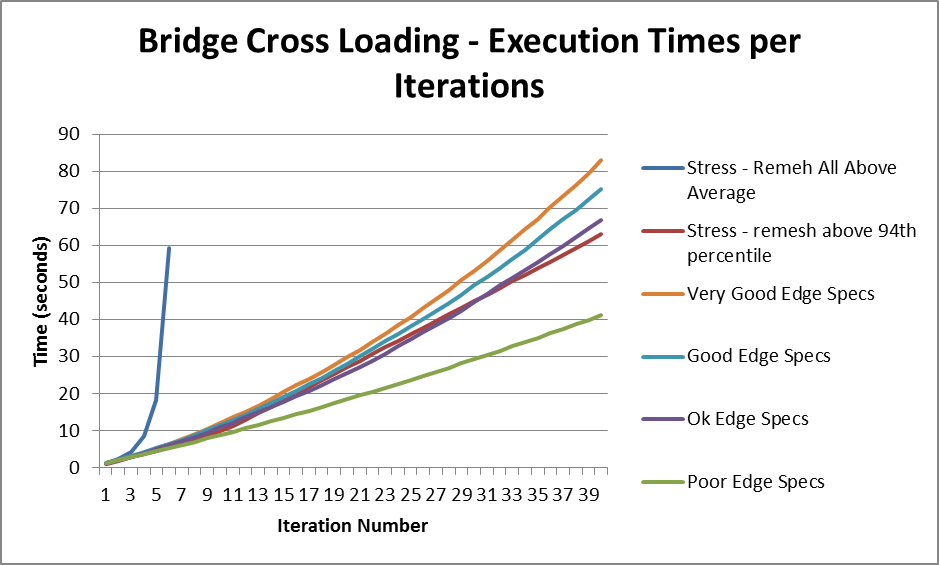
\includegraphics[width=0.9\linewidth]{../Graphics/Graphs/BridgeCrossLoadingExecutionTimesPerIterations.png}
  \caption{Execution time in seconds for each method to reach 40 refinement iterations}
  \label{fig:sub1}
\end{subfigure}%
\begin{subfigure}{.5\textwidth}
  \centering
  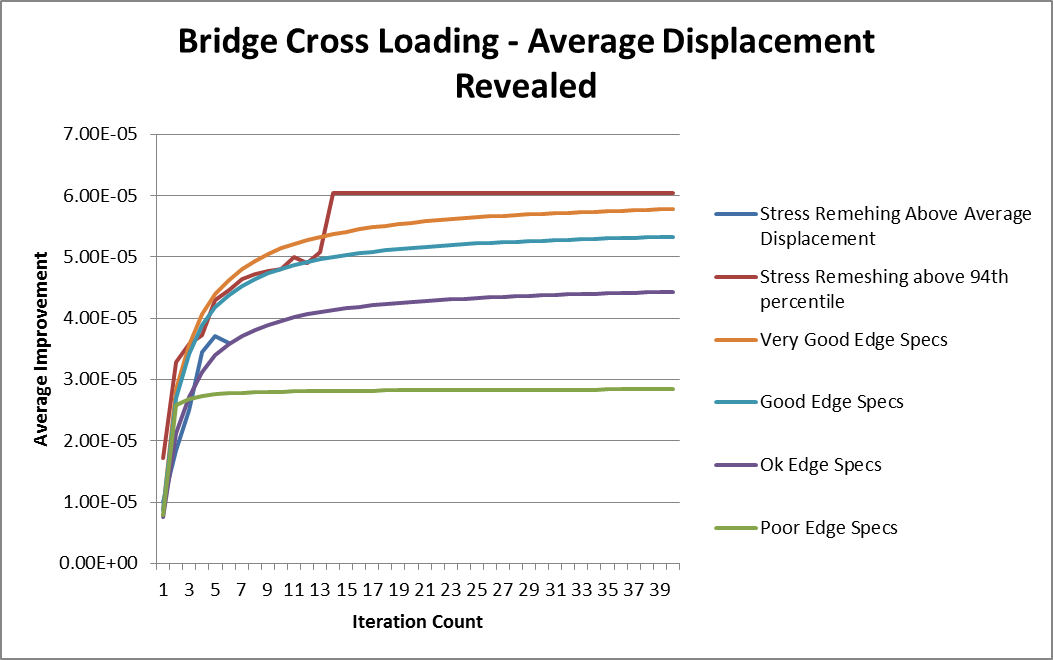
\includegraphics[width=0.9\linewidth]{../Graphics/Graphs/BridgeCrossLoadingAverageDisplacementRevealed.png}
  \caption{Average amount of displacement and thus stress revealed by each approach as number of iterations increases}
  \label{fig:sub2}
\end{subfigure}
\label{fig:test}
  \caption{Execution time increase compared to the amount of information revealed for the different approaches}
 \end{figure}

\noindent
For stress refinement the varied parameter was the threshold used to determine whether elements were considered under high stress and should be further refined. The main consequence of varying this parameter was change in both the node count and the programs runtime as can be seen in Figure 14a. Despite time complexity for subdivision being $O(n^2)$ for all methods using a low threshold results in large values of n and consequently a rapid increase in both runtime and element count. \\

\noindent
In order to perform a reasonable comparison between both the stress and heuristic refinement methods it was important to specify the threshold such that approximately equal amounts were performed by each approach per unit of weighting for each iteration (see combining methods under System Design), thus allowing each method to be evaluated on its merit to select elements appropriately and a hybrid method through its designated weightings. To do this the increase in element count was tracked for the different heuristic methods, as can be seen in Figure 10. The average increase in elements per iteration could then be calculated as 6\% of the total number of elements within the model. This meant stress refinement could be reasonably compared to heuristic refinement if for each use of the refinement it only re meshed those elements considered to be above the 94th percentile in terms of stress. \\ 


\begin{figure}[!h]
  \centerline{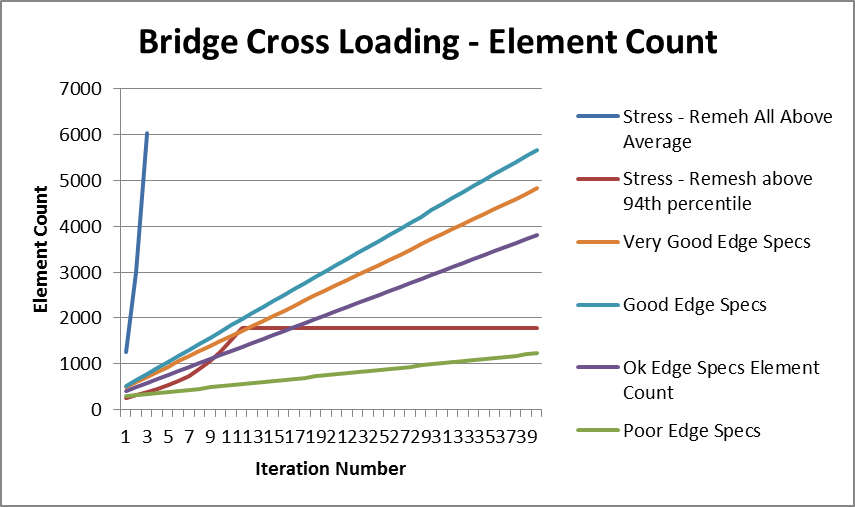
\includegraphics[width=110mm, scale=1]{../Graphics/Graphs/BridgeCrossLoadingElementCount.png}}
  \caption{Increase in element count for the various refinement methods over forty iterations}
  \label{fig:sub1}
\end{figure}

\noindent
%Having obtained data from multiple runs of the individual methods 
Executing the bridge model for a variety of hybrid weightings revealed the following general trends in the amount of stress discovered per iteration:

\begin{figure}[!h]
  \centerline{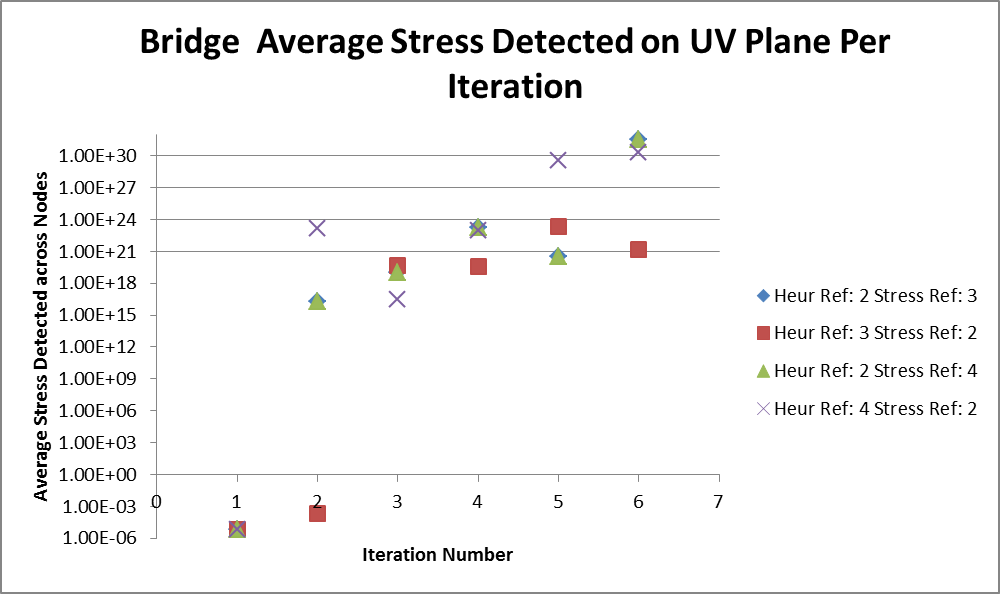
\includegraphics[width=110mm, scale=1]{../Graphics/Graphs/BridgeCrossLoadingAverageStressRevealed.png}}
  \caption{Increase in element count for the various refinement methods over forty iterations}
  \label{fig:sub1}
\end{figure}



\begin{figure}[h!]
\centering
\begin{subfigure}{.5\textwidth}
  \centering
  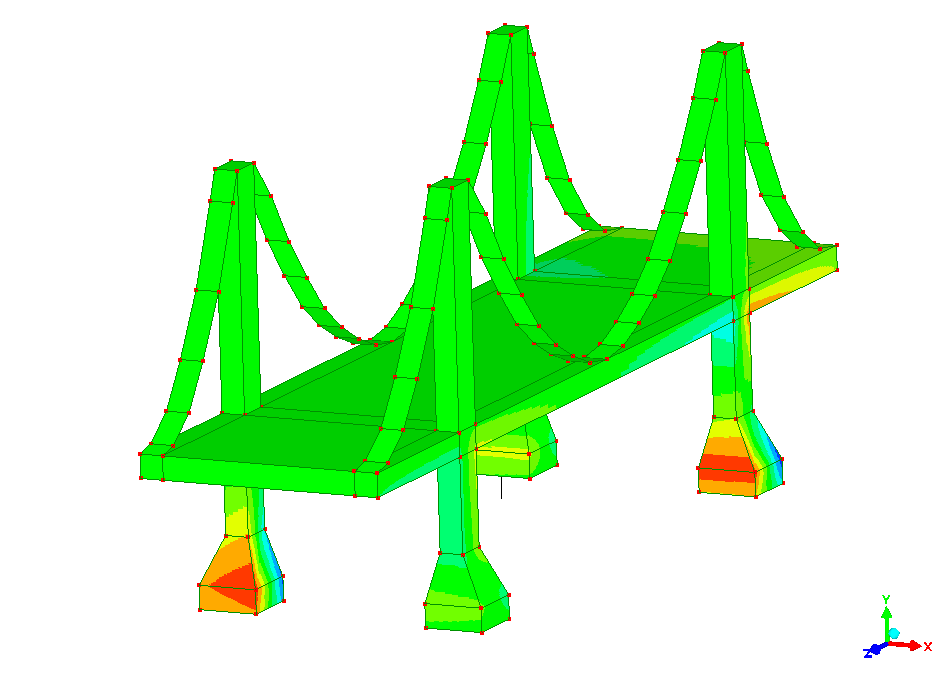
\includegraphics[width=0.9\linewidth]{../Graphics/BridgeCrossLoadingStress/bridgeStressBasic.png}
  \caption{Stress Revealed through the initial highly coarse bridge mesh without running any iterations for either method}
  \label{fig:sub1}
\end{subfigure}%
\begin{subfigure}{.5\textwidth}
  \centering
  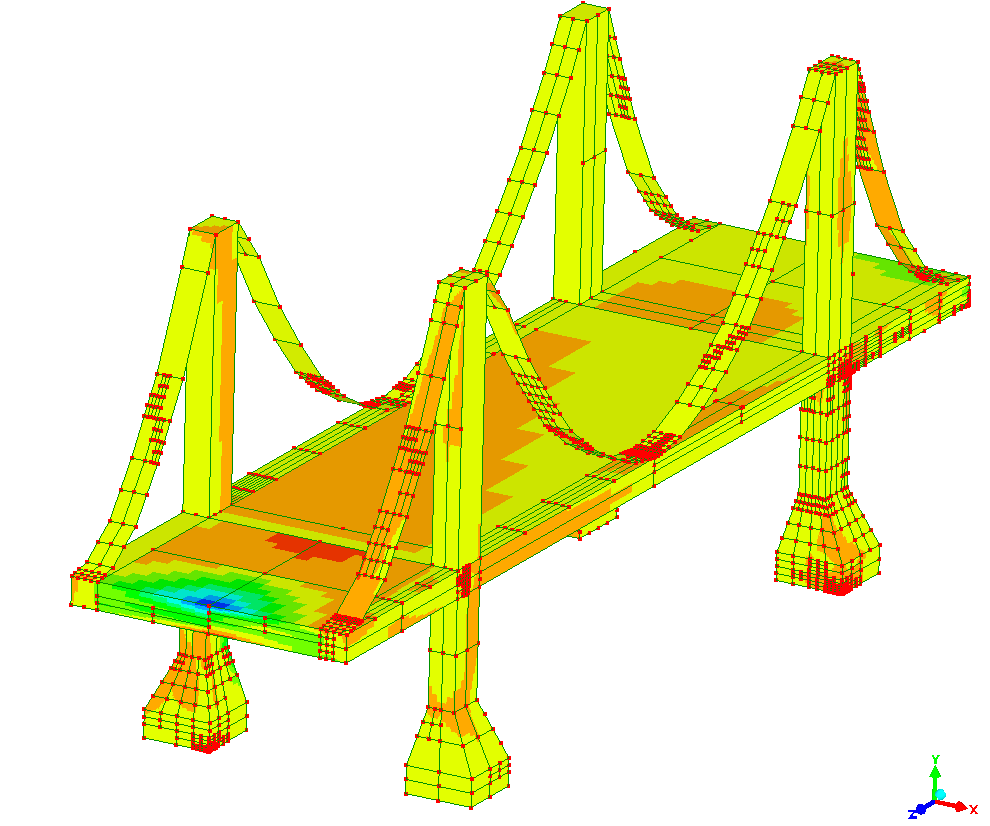
\includegraphics[width=0.9\linewidth]{../Graphics/BridgeCrossLoadingStress/Hybrid-best-3-2.png}
  \caption{Stress revealed within model after just 4 iterations with a heuristic stress method weighting of 3-2, edge heuristics also considered good in this case}
  \label{fig:sub2}
\end{subfigure}
\label{fig:test}
  \caption{Execution time increase compared to the amount of information revealed for the different approaches}
 \end{figure}


Looking at the metric and the resulting meshes it is clear that the system very quickly identifies areas under very high stress with both of the two approaches, with meshing being highly focused on those areas and consequently a rapid increase in the average stress covered by the elements in the model after only two iterations. 

%say something about how actually you want a bit of distribution

\noindent
Comparing the amount of improvement performed by both the stress and heuristic refinement processes with varying weightings that in general heuristics performed better than stress refinement although interestingly more weighting did not necessarily correlate to better results as can be be seen with heuristic weighting of two doing a better job than weighting four in the final iteration. \\


\begin{figure}[!h]
  \centerline{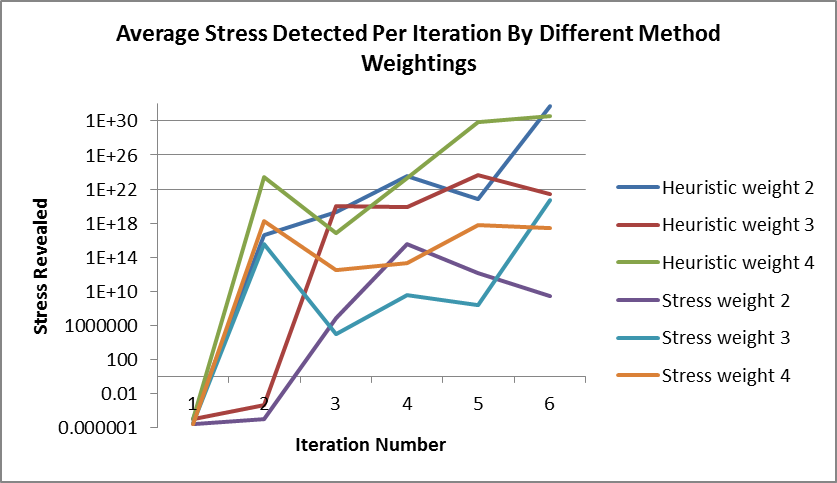
\includegraphics[width=110mm, scale=1]{../Graphics/Graphs/AverageStressDetected Per Iteration By Different Method Weightings.png}}
  \caption{Increase in element count for the various refinement methods over forty iterations}
  \label{fig:sub1}
\end{figure}



\begin{figure}[!h]
  \centerline{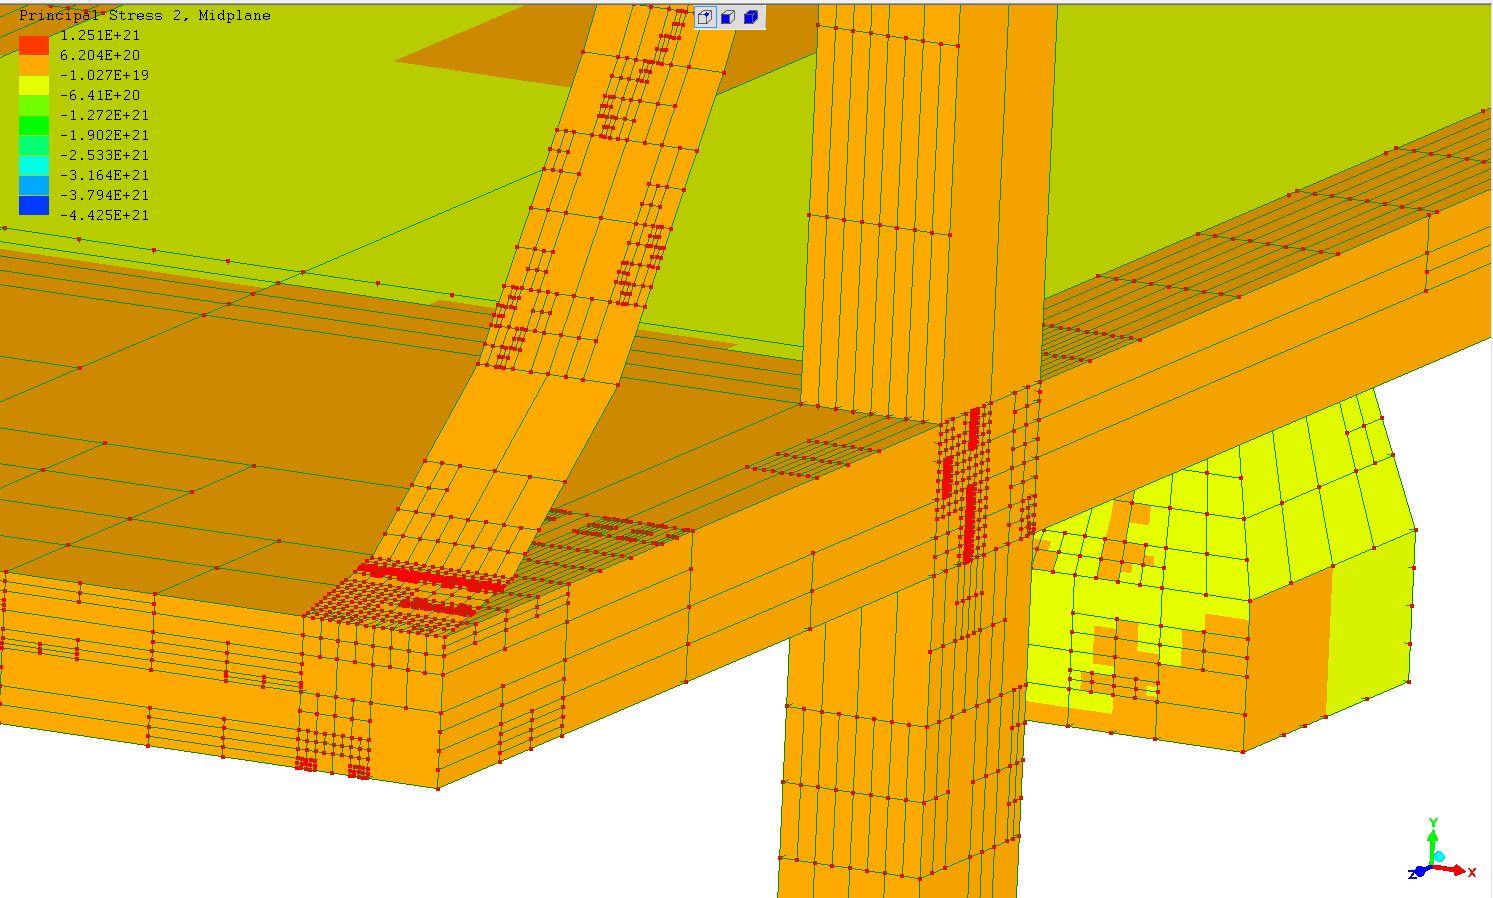
\includegraphics[width=110mm, scale=1]{../Graphics/BridgeCrossLoadingStress/BridgeCrossLoadingStress6-3-2.png}}
  \caption{Intense meshing occurring around stress points at joint intersections}
  \label{fig:sub1}
\end{figure}


\noindent
Effective comparison of the two methods indicates that the system works as a tool by which comparisons of different refinement methods can effectively be made. 

%


\subsubsection{Evaluation Issues}
A significant issue faced in attempting to demonstrate the effectiveness of the system was to provide an indication of how well the system worked without taking into account the ability of the user who may be providing the edge rules for a particular model. Not taking this into account would result in an inaccurate representation of its ability.

\subsection{Strengths and Weaknesses}
The resulting system successfully satisfied both the functional and non functional requirements in addition to providing insights into the possibilities of a hybrid technique for effective finite element meshing, something that was optimistic at the start of the project but highly desirable. The project was well managed with all of the objectives being delivered as per the initial time plan. Quality was also maintained throughout the project by the application of good software engineering practice. \\

\noindent
One of the great strengths of the finished system was its modular architecture which allows for a great amount of potential extendibility in the future. Although little focus has so far been given to the systems usability it could be developed and distributed as a public tool for experimentation with hybrid meshing with limited additional effort. \\

\noindent
Another strength of the system is its ability to accept any heuristic definition in terms of edges within a mesh structure. Theoretically this means the final system is also capable of using the same types of edge specifications for any type of FE analysis such as fluid flow or heat transfer given a corresponding rule set by which to mesh with. \\


\noindent
A downside of the current design is the need for the user to manually specify the edges by the user directly into the JSON input file which is both time consuming and prone to error despite the relatively small size of the models analysed in this dissertation. Comparing the size of these with those used in industry it is clear that this process is simply not practical for engineers conducting FE analysis. To change this better tools are required that will allow engineers to automatically generate edge specifications quickly, most likely through some GUI or a bespoke high level language capable of combining knowledge about the mesh structure and different types of edges to generate specific rules. Again this is beyond the scope of the project and would likely be a dissertation in its own right. \\


\noindent
Although the system had a strong subsystem and class level architecture many of its weaknesses could be attributed to needing to prioritise the ability to perform rapid prototyping over efficient implementation of the various algorithms and methods described in this dissertation. Much of this a consequence of overusing the functional programming capabilities within the C\# LINQ library. Widespread adoption of functional programming practices was stated as a desirable aspect of the final system implementation within the non-functional requirements. This has largely been adhered to with  higher order and lambda functions widespread throughout the codebase. In the later stages of the project it became apparent however that in many cases reliance on these features resulted in reduced readability and performance for many of underlying algorithms described in this dissertation. \\


% Overall the project met all its initial requirements laid out in both the objectives and its requirements.
% Sould have done test driven development to ease testing at the end


\subsection{Evaluation summary}
